%%%%%%%%%%%%%%%%%%%%%%%%%%%%%%%%%%%%%%%%%%%%%%%%%%%
%% P3: Phenomenology of Particle Physics                         
%%
%% Author:  André Rubbia                   		 
%%
%% Figure 3.6 Concept of a collider compared to a fixed target configuration. 
%%
%% This work is licensed under the Creative Commons Attribution 4.0 International License. 
%% To view a copy of this license, visit http://creativecommons.org/licenses/by/4.0/ or 
%% send a letter to Creative Commons, PO Box 1866, Mountain View, CA 94042, USA.
%%
%%%%%%%%%%%%%%%%%%%%%%%%%%%%%%%%%%%%%%%%%%%%%%%%%%%

\documentclass[a4paper,10pt]{article}

\usepackage[T1]{fontenc}
\usepackage[utf8]{inputenc}
\usepackage{lmodern}
\usepackage[labelfont=bf]{caption}
\usepackage{upgreek}

\usepackage{tikz}
\usetikzlibrary{patterns}
\usetikzlibrary{decorations.pathmorphing}
\usetikzlibrary{decorations.markings}
\usetikzlibrary{arrows}
\usetikzlibrary{svg.path}
\usetikzlibrary{shapes}
\usetikzlibrary{arrows.meta}
% define the arrow style
\tikzset{
    arrow/.style={
        decoration={
            markings,
            mark=at position .5 with {
                \arrow[#1, scale=1.5]{latex}
            }
        },
        postaction={decorate},
    }
}
\tikzset{
    arrow flipped/.style={
        decoration={
            markings,
            mark=at position .5 with {
                \arrow[#1, scale=1.5]{latex reversed}
            }
        },
        postaction={decorate},
    }
}
\pgfkeys{/pgf/number format/.cd,1000 sep={}}\usepackage{pgfplots}
\pgfplotsset{compat=1.17}
\usepgfplotslibrary{ternary}
\usepgfplotslibrary{fillbetween}
\usepgfplotslibrary{external}

\def\d{\mathrm{d}}

\begin{document}

%%%%%%%%%%%%%%%   FIGURE  %%%%%%%%%%%%%%%%%%%%%%%%%%%%%%
\begin{figure}[htb]
\begin{center}
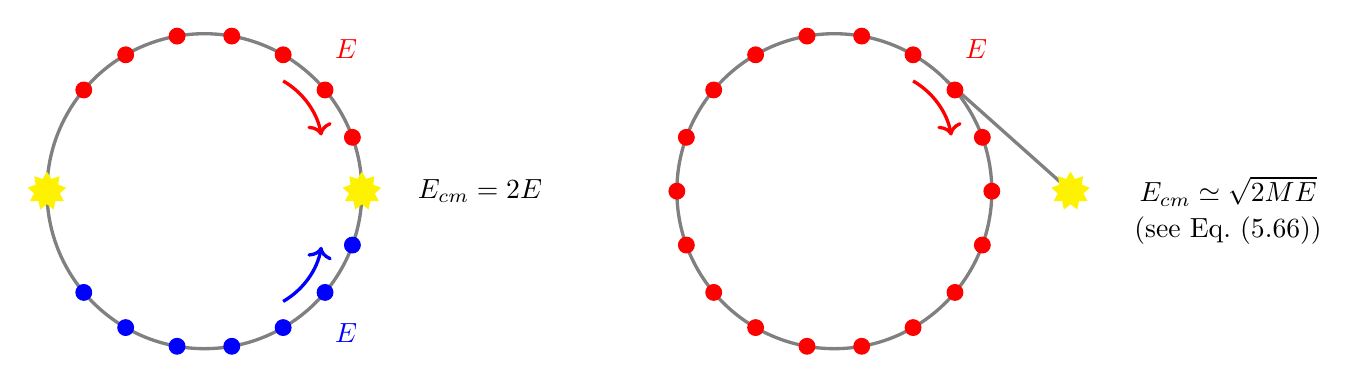
\begin{tikzpicture}[scale=2.0]
	\begin{scope}[shift={(0,0)}]
	    \draw[very thick, color=gray] circle (1.0);
	    \node[fill,color=yellow,star,star points=9,minimum width=0.2] at (-1,0) (0.1) {};
	    \node[fill,color=yellow,star,star points=9,minimum width=0.2] at (1,0) {};

	   \foreach \x in {20,40,60,80,100,120,140}
	   	 \draw[fill,color=red]  ({cos(\x)},{sin(\x)}) circle (0.05);
	   \foreach \x in {-20,-40,-60,-80,-100,-120,-140}
	   	 \draw[fill,color=blue]  ({cos(\x)},{sin(\x)}) circle (0.05);

	    \draw[red] node at (0.9,0.9) {$E$};
	    \draw[blue] node at (0.9,-0.9) {$E$};
	    \draw[black] node at (1.75,0) {$E_{cm}=2E$};

	   \draw[very thick,->,red] (0.5,0.7) arc (60:10:0.5);
	   \draw[very thick,->,blue] (0.5,-0.7) arc (-60:-10:0.5);
	\end{scope}
	\begin{scope}[shift={(4,0)}]
	    \draw[very thick, color=gray] circle (1.0);
	    \draw[very thick, color=gray] (0.707,0.707)--(1.5,0);
	    \node[fill,color=yellow,star,star points=9,minimum width=0.2] at (1.5,0) (0.1) {};

	   \foreach \x in {0,20,40,60,80,100,120,140,160,180}
	   	 \draw[fill,color=red]  ({cos(\x)},{sin(\x)}) circle (0.05);
	   \foreach \x in {-20,-40,-60,-80,-100,-120,-140,-160}
	   	 \draw[fill,color=red]  ({cos(\x)},{sin(\x)}) circle (0.05);

	    \draw[red] node at (0.9,0.9) {$E$};
	    \draw[black] node at (2.5,0) {$E_{cm}\simeq \sqrt{2ME}$};
	    \draw[black] node at (2.5,-0.25) {(see Eq.~(5.66))};

	   \draw[very thick,->,red] (0.5,0.7) arc (60:10:0.5);
	\end{scope}
	    \end{tikzpicture}
	\caption{Concept of a collider (left), compared to a fixed target configuration (right).}
\end{center}
\end{figure}
%%%%%%%%%%%%%%%   END FIGURE  %%%%%%%%%%%%%%%%%%%%%%%%%%%%%%

\end{document}
